\section{C}
This section deals with the basics of C and things you will using a lot in C.
\subsection{Data Types}
There are three major types of data in C; int, float, and char.
\paragraph{int} Integers in C are 32-bits long, represented by the 2's compliment system, so they can represent values $[-2^{31}, 2^{31} - 1]$. You can use \textbf{unsigned int}, which removes the negative from the int, representing values $[0, 2^{32} - 1]$. If we wanted to represent larger numbers, we can use \textbf{long long int}, which is 64-bit int with values $[-2^{63}, 2^{63} - 1]$
\paragraph{float} Floats in C are of size 32-bits; they are represented in IEEE 754 single precision, hence 15 and 15.0 have different representations. The range of a float is $[1.401298x10^{-45}, 1.401298x10^{38}]$. We use \textbf{double} for 64-bit long double precision values.
\paragraph{char} Chars are 1-byte integers. It uses 8-bit ASCII encoding to represent characters.
\paragraph{Memory Allocation} Each data type is allocated memory of its respective fixed size. When allocated, there is a garbage value until a value is assigned. Constants, declared as \textbf{const} are stored in read-only memory, causing errors when attempting to change the value. Pointers have a size of 4 bytes.
\subsection{Function Calls and Scope}
\paragraph{Functions} Function calls are executed on the stack. For each function call, a stack frame is allocated. The stack grows upwards from low addresses to high addresses. The scope of values is within their own function, so a value initialized in one function is out of the scope of another function. However, with the nature of the stack, sometimes  uninitialized 'garbage' values are not so garbage. This is because the second function is in the same location in the stack as the previous function, so if they have the same types of variables, they could inherit the same value. This can be seen in the figure, where the \textbf{d} is initialized with the value of \textbf{a}. \newpage
\begin{figure}[!htb]
	\center{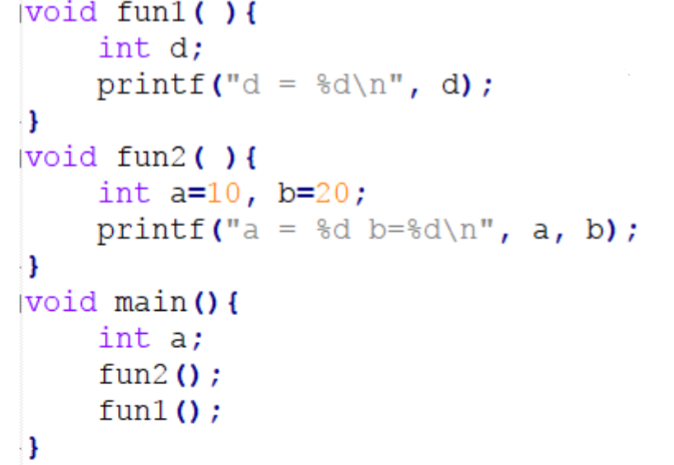
\includegraphics[width=7cm]
		{c/functioncall}}
	\caption{\label{fig:functioncall} Function examples}
\end{figure}
\paragraph{Recursion} Recursion is possible in C. At a low level, each recursive call creates a new stack frame. If there is no stop condition, and with the usual finite stack, there will be overflow and the program will crash.
\paragraph{Preprocessor Directives} The $\#$ used at the start of a C file is referred to as a C preprocessor directive. They allow the inclusion of:
\begin{itemize}
	\item Header Files
	\item Macro Expansions
	\item Conditional Compilation
	\item Line Control
\end{itemize}
A macro is a fragment of code which has been given a name. \textbf{\#define NAME tokens} Think in the style of finals or constants; you can do \textbf{\#define MAX 100} and use the word MAX in the rest of your code, the compiler will switch out the macro with the value it is defined as. You can also define functions in macros, but should be used for basic functions like multiplying two values and returning the result.
\subsection{Arrays}
An array is a data structure that stores a fixed sized, sequential collection of same typed elements. Arrays start at 0, and increment. In memory, they are stored, unsurprisingly, from low address to high address. This is because arrays are accessed by taking the base address and adding onto it the index with the distance between addresses of the object. (eg, an object of 32 would have addresses 0, 32, 64, etc.) \newline
Arrays can be accessed with a[index], where a is the name of the array. In C, $a$ cannot be assigned to anything. It is equivalent to $\&a[0]$, the address of $a[0]$. Doing $^*\&a[0]++$ is the same as $a[1]$. Passing an array to a function is simply just passing the address of its first value, similar to a pointer if you will. You also can't return an array, so you either have to change the values directly in the address or return a pointer. 
\newline A note, the compiler does not know the size of an array during compile time, so arrays can potentially lend themselves to creating potential issues in your code. Array sizes also can't be dynamically changed. When two arrays are created one after the other, the 2nd array address is directly after the end of the 1st array, similar to initializing two variables of any type. Since array access isn't checked and garbage isn't collected, you can access values you don't mean to access with an array.
\subsection{Pointers}
\paragraph{Pointers} A pointer is an address variable. It stores the address of a data item. The type of the pointer is the type of the object it points to. Data pointers have size of 4 bytes in a 32-bit system and size of 8 bytes in a 64-bit system. When using pointers, there are two key characters we need to understand; \textbf{'$^*$'} and \textbf{'\&'}. $^*$ is used to declare pointers and obtain the value its pointing to. \& is used before a non-pointer variable to obtain its memory address. This can be seen in the figure.
\begin{figure}[!htb]
	\center{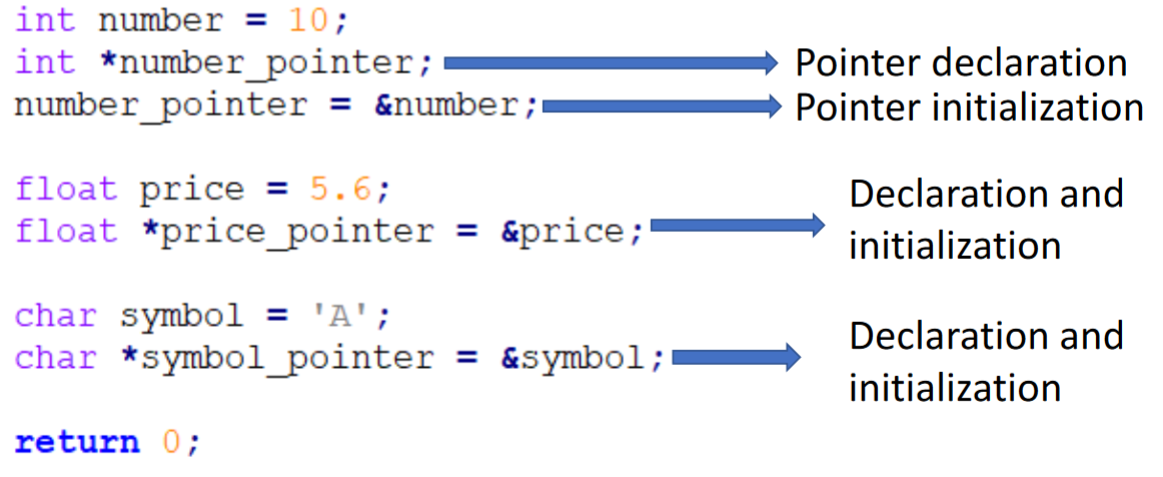
\includegraphics[width=13cm]
		{c/pointers}}
	\caption{\label{fig:pointers} Pointer Declaration and Initialization}
\end{figure}
\newline
One way to think of pointers vs variables, is to think of a variable as something that contains stored data and requires a symbol to obtain its address, whereas a pointer is something that contains an address and requires a symbol to obtain its stored data. Multiple pointers can point to the same address, and this can be used to pass data into functions.
\paragraph{Pointers in Functions} When passing variables into a function, it does not pass the declared variable, instead it passes the data into a new memory address, so assignments in the function will not change the variable passed in during the function call. However, using the magic of pointers, we can change that. Instead, all we have to do is pass the memory of the variable, and in the function create a pointer that points to that address and change its value by obtaining it from our pointer. This nifty trick is how we pass arrays into a function. An example is seen below. The final values of x and y in the main function will be 10 and 4, respectively.
\begin{verbatim}
	void foo(int *x, int y) 
    {
        (*x)++;
        y++;
        return;
    }
	
    int main()
    {
        int x, y;
        x = 9;
        y = 4;
        foo(&x, y);
	
        return 0;
    }
\end{verbatim}

You can also return pointers from functions. This is simple to do.
\begin{verbatim}
    int *foo()
    {
        int x = 10;
        int *p = &x;
        return p;
   	}
\end{verbatim}

There is also some syntax to be careful of with pointers. For example, ($^*$p)++ and $^*$p++ are not the same thing. The first one first pulls the value stored in the pointer's memory, and applies '++' to the value. The second one increments the memory address first, then pulls out the value stored in the memory. Parenthesis are important!
\paragraph{Type of Pointer} When pulling a value out of a pointer, it's takes the appropriate amount of bits it needs from the memory address pointed to. So if you have a char pointer pointed to an integer, it will pull some bits from the int and represent it as a char. In addition, when increment the pointer with p++, it will scale it's memory address based on the type its pointing to. p+1 is the same as p + 1*scaling\_factor, this scaling factor is based on the size of the type the pointer is pointing to. This is behavior seen in arrays.
 
\paragraph{Arrays and Pointer Movement} It is important to realize that arrays are simply pointers, as mentioned earlier. If we have a pointer p = \&a[0], then doing $^*p++$ is the same as $a[1]$. As such, pointers can end up pointing to places we probably don't want it pointing. Pointers can also be added together, subtracted, etc. What it does is offset the memory address based on the operation. Messing around with addresses can easily lead to broken, buggy code, but it's still useful for managing code.

\paragraph{Allocating Memory} When declaring arrays and pointers, it will allocate memory, but we don't always know how much memory we want to allocate, or perhaps we want to do it sort of in code to not be wasteful. How do we set aside memory for a pointer or array? How do we free up our memory once we are done with the data? This is easily achieved by using the functions malloc and free. \newline
\textbf{malloc(size)} allocates a space in memory equal to the size passed in, and returns the address of the first position in memory allocated. If there isn't enough space in memory for allocation, it will return a null value. You can check for the pointer assigned with its address if it is null or not to manage the code. This memory is obtained from the heap.\newline 
Finally, to free up space, all we need to do is do a good old \textbf{free(pointer)} command, and it will free all memory associated with that pointer or array and return back to the usable/free heap for later mallocs. The pointer will then have garbage value, so it is suggested to set it to null and do null checks to ensure the free went through later and avoid odd bugs caused from freeing. This also helps to be mindful of double free errors, where we free the same pointer twice. This causes the address of the pointer to be seen as "free" for allocation twice, meaning it can be allocated later, and then replaced without being freed.

\subsection{User Defined Types}
C doesn't have objects. So how are we supposed to do things that work super well in user defined object form? Oddly specific question, but there is an oddly specific answer. C has the ability to create \textbf{struct} and \textbf{union} instead of classes.
\paragraph{Structs} Assume we have a table of students, with their name, id number and their marks. These values all have different types (char*, int) but they can be logically grouped. We can create our own type and call it struct. Let's get some definitions out of the way. Structs are used to pack logically related data items and can be treated as a single item. Think of them as a data container. The data items packed in a struct are referred to as members. These members can be of different types. They can even be structs!
\begin{figure}[!htb]
	\center{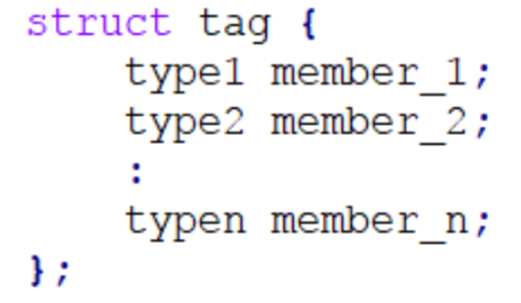
\includegraphics[width=4cm]
		{c/createstruct}}
	\caption{\label{fig:structdeclare} Declaring a new struct}
\end{figure}
\paragraph{Memory Allocation} The layout of a struct in memory is fairly straightforward. Structs in memory are allocated the size of each member in the order they are declared in the struct. This can result in some padding, for example one char followed by a pointer could result in threes byte being wasted/padded, if we assume the pointer to need be in a multiple of 4. (This is because the char takes index 0, and index 3 is the next multiple of 4, so the three bytes are padded to allow the pointer to be allocated in the same general area as the char in the struct).
\paragraph{Struct Pointers} Structs are treated like a data type, so you can create a pointer for a struct. The syntax is as follows, \textbf{struct tag *p}. A note here is that all structs need the word "struct" before their name. You can avoid this by adding \textbf{typedef struct tag TAG}. This defines out "struct tag" as just "TAG" for all uses, allowing us to declare variables as \textbf{TAG *p}. Less verbose, so its usually a good idea.
\paragraph{Accessing Members} There are two ways to obtain the member from a struct. Assume we have a struct in the variable "t1" and the pointer "p" and has a member "name". You can access it using the usual way to access public variables in the likes of Java; as \textbf{t1.name}. With a pointer, however, there are two ways to accomplish this. You can get the value out of a pointer and access using a period from there; \textbf{($^*$p).name}, but there is a shorthand way. You can just do \textbf{p $\rightarrow$ name}. It's less to type, and is equivalent to the period syntax.
\begin{figure}[!htb]
	\center{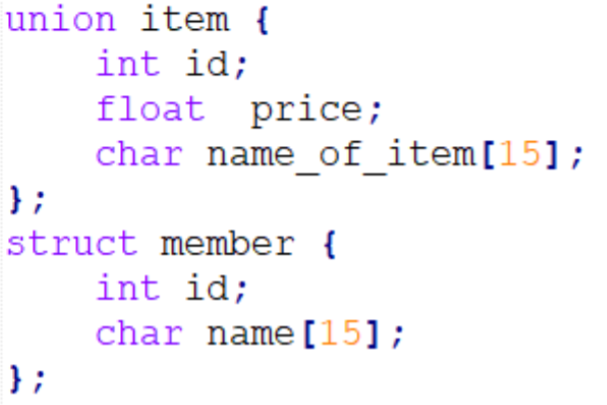
\includegraphics[width=4cm]
		{c/unionstruct}}
	\caption{\label{fig:unionstruct} Struct VS Union }
\end{figure}
\paragraph{Unions}
Unions are similar to structs. They have names, can be typedef'd, contain members and all that stuff. They differ from structs in how it appears in and manages memory. Where structs allocate memory for each of its members, unions only allocate as much space as their largest member, with some potential padding. As seen in the figure, the struct has size at least 19, whereas the union will be smaller at size at least 15, the size of its largest member, despite having a combined size of 23.

\paragraph{Nested Types} A special note, a struct/union cannot contain a member variable of their own type. However, a neat work around is that you can have a member that is a pointer to its own type. Using these pointers, you can create recursive data types such as binary trees and linked list. We did an assignment on this, and it is best to look back at that for specifics on how to implement such features. 

\subsection{Optimization}
When we talk about optimization, there are really three different directions we can take, and the desired direction is dependent on context. We have flexibility, time, and space.
\begin{itemize}
	\item Flexibility: How flexible is our code? How many different situations can it handle, and how well can it handle them?
	\item Time: How fast does our code achieve what it was meant to achieve? Can it be \textit{even faster?}
	\item Space: How much memory does our program use it any one time? Can we reduce it without changing what it was meant to do?
\end{itemize}
In an ideal world, we would optimize all three to their full extent. Sadly we don't live in an ideal world, so some sacrifices in some areas have to be taken to optimize for others. 
\paragraph{Speed Optimizations} When it comes to speed, we can compare speed by using ratios. $\frac{Speed_{old}}{Speed_{new}}$ and speed is usually a measure of time from the start of the function or program to the end. Ofcourse, this just tells us how to measure time, but how do we actually improve the speed of our programs? There are many ways to go about this, but the first step is to identify costly functions. The simplest example would be looking at two functions, one that adds matrices and the other that subtracts them. The matrix multiplication has a higher complexity, so it could be a cause for concern.\newline
Speed optimization tactics:
\begin{enumerate}
	\item Use a better algorithm: Straight-forward, some algorithms are just faster.
	\item Use inline functions: For small functions, we can macro them and let the compiler just apply the function's operations without the overhead in the stack from function calls. You can achieve this using the "inline" declaration instead of a macro, in fact inlines are usually preferred. Be careful when inlining larger or more complex functions, because inlining could then just make a giant compiled code that takes more space and has higher load times.
	\item Loop unrolling/jamming: Loops add an overhead on their check conditions on each iteration. You can reduce this by going through multiple iterations at once (5 at a time instead of 1). You can also attempt to combined two loops together even though they might do different things. Since they both will loop, combining into one completely removes the loop overhead from one of them; this is called loop jamming.
	\item Pass by references: Passing by values is slower than passing by references, because new memory is allocated for the new values and things like this take time (and additional space!)
	\item 5. Avoid recursion: Recursion kills your (stack) frames
	\item Avoid dynamic memory allocation: Constant access and change in memory results in slow access operations, as well as overhead from the memory manager knowing which heap space is used up or free.
\end{enumerate}
These are just some optimization techniques. In practice, code optimization is on a code to code basis.

\section{C++}
This section deals with features in C++ and why its used more than C.
\subsection{Introduction}
\paragraph{C++} C++, as the name suggest, is an increment to C. While it has all of the features C has, it also has some bonus features. It's primary purpose is to make C an object oriented programming language, adding classes, constructors/destructors, and various other features for polymorphism and memory management.
\paragraph{Reference Variable} One thing we can do in C++ is creating a reference variable. Reference variables are similar to pointers in that you can pass them into functions to pass by reference, but you do not need to dereference it with ($^*$p), as it is already dereferenced by nature. This allows you to bypass on using pointers in the case you only want to pass a reference variable. The syntax to declare a reference is \textbf{int \&r}; much like declaring a pointer type but using \& instead of *.
\paragraph{Overloaded Functions} In C, a function's signature is its name, so you cannot have two different functions with the same name even if they had different parameters. This is not the case with C++. A function's signature is comprised of three things.
\begin{enumerate}
	\item Name
	\item Number of Parameters
	\item Type of Parameters
\end{enumerate}
Meaning the functions \textbf{void foo()} and \textbf{void foo(int a)} have different signatures. Note that the return type of a function is not a part of its signature, meaning \textbf{int foo()} and \textbf{void foo()} have the same signature and will cause an exception.

\paragraph{Classes} C++ has the ability to have classes for the object-oriented programming. When declaring a class, you can define members and functions in either the private or the public region. By default, members and functions are private, so the private region can be omitted. 
\begin{figure}[!htb]
	\center{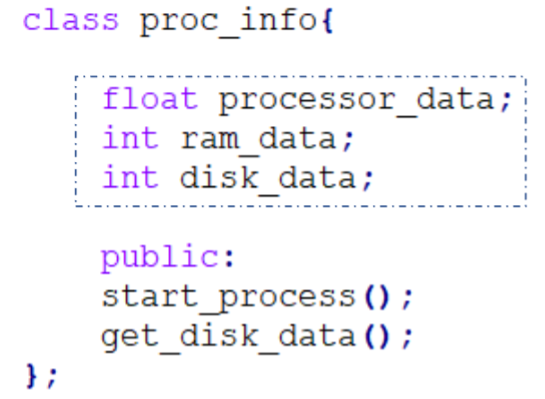
\includegraphics[width=6cm]
		{c/classes}}
	\caption{\label{fig:classes} Private members and public functions example}
\end{figure}
\paragraph{Constructor} C structs are not exactly objects. They cannot be initialized at time of declaration, they have to done at separate lines. C++ classes, on the other hand, can be initialized at time of declaration. We do this using constructors. Constructors are a special member function that has the same name as the class. In the body of the constructor method, we can initialize values to default, or accept them from an input. The syntax for a constructor is the same as any other method, but the name has to be the same name as the class.
\paragraph{Copy Constructor} A copy constructor is one that receives a reference to its own class as a parameter, such as \textbf{class(class \&c)} as a constructor. You CANNOT pass in the value of the class, it has to be by reference. You can then access the passed in reference and copy the values as you see fit, as if it ws any other method.
\paragraph{Destructors} A destructor is a special member function whose name is the same as the class with a $\sim$ appended behind it. \textbf{$\sim$ class()}. Destructors are called in two instances; when a temporary object passes out of its scope, and when we use the "delete" operator (next section). It is the responsibility of the programmer to deal with what happens in the destructor.
\paragraph{New and Delete} C++ introduces two operators we can use for managing memory; \textbf{new} and \textbf{delete}. These are used to manage dynamically allocated memory; new is for declaring memory blocks and delete is for freeing memory blocks (similar to malloc and free). Using new allows us to initialize and declare an object at the same time, while delete explicitly calls the destructor and does whatever you need it to do.
\subsection{Inheritance}
\paragraph{Operator Overloading} C++ aims to make user defined classes almost the same as built in types, like int. One of things we can do with built in types is manipulate them with operators, like \textbf{+} - r\textbf{-}. User defined classes don't have these operators by default, so we have to define them ourselves. We do this using a special method referred to as an operator function. For example, if we wanted to define \textbf{+} for our class, we would declare our function's return type as its own class, and the function's signature would look like \textbf{operator +(class c)}. This is results in the following to mean the same thing/
\begin{itemize}
	\item c$\_$sum = c1 + c2;
	\item c$\_$sum = c1.operator+(c2);
\end{itemize} 
The left hand side calls the function with the right hand side as the argument. You can also have operators without arguments, such as negation (-c1).
\paragraph{Friend Function} What if we wanted to add a float with our own class? This is easy if we use the float as the argument as \textbf{operator +(float f)}. But what if the float is the one calling its own function? We can't just redefine the operators in the float data type, so we need to use a different method, called friend functions. Friend functions are defined outside of the class scope, but it has access to all private and protected members of a class. Our \textbf{operator +(float f)} can now be defined as \textbf{friend operator +(class c, float f)} and we can now add in when our argument is float on the left as \textbf{friend operator +(float f, class c)} Note: the overloaded operator function must have at least one operand of the class it is in.
\paragraph{Inheritance} Classes in C++ can inherit from one another, much like in java. There are a few types of inheritance to cover in C++.
\begin{itemize}
	\item Single Inheritance: A derived class inherits from a single base class
	\item Multiple Inheritance: A derived class inherits from more than one base class
	\item Multilevel Inheritance: A derived class inherits from another derived class; like a chain.
	\item Hybrid Inheritance: A wombo combo of other inheritances
\end{itemize}
\begin{figure}[!htb]
	\center{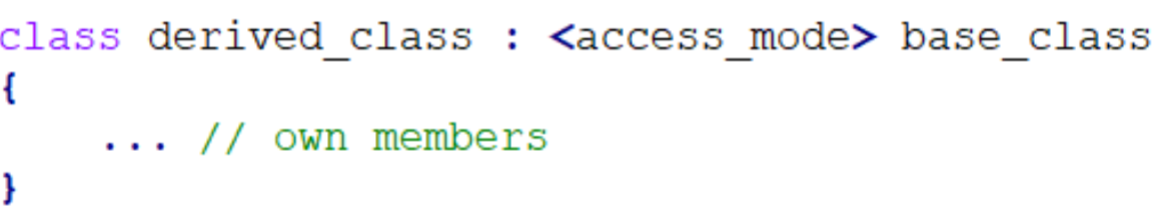
\includegraphics[width=12cm]
		{c/inheritance}}
	\caption{\label{fig:inheritance} Syntax for Single Inheritance}
\end{figure}
\paragraph{Visibility} Access mode, as seen in \figurename{inheritance}, can either be private or public, with the default being private. If it is public, then the public members of the base class are inherited as public members, otherwise the inherited members become private. When doing multiple inheritance, the syntax is the same as for one base class, but we separate the multiple base classes with commas. Note: private members of base classes are not inherited! \newline
Now what if we wanted to inherit something, but we didn't want it to be public in the base class? There is a third visibility identifier we call "protected." Protected members are public for its children, but are private for all other areas. Access mode can also be protected in inheritance declaration. 
\paragraph{Virtual} Sometimes, we can accidentally inherit functions with the same signatures from different classes. What we can do is declare functions as virtual. Virtual functions are ones that are expected to be overridden in their child classes (similar to abstract in Java, but they still function as normal in the parent class) You can also declare parent classes to be virtual, this helps to stop multiple copies of the same grandparent to be created.

\subsection{Memory Management}
\paragraph{C vs C++}
C provides \textbf{malloc(), calloc(), realloc()} for dynamic memory allocation, and \textbf{free()} for dynamic memory deallocation. C++ provides \textbf{new} for ynamic memory allocation, and \textbf{delete} for dynamic memory deallocation. C++ provides some additional bonuses too, it provides the manual memory management as we have seen so far, but it can also provide the convenience of garbage collection when desired. We get garbage collection C++ using smart pointers.
\paragraph{Smart Pointers} 
\paragraph{Rule of Five}

\subsection{Templates}
templates
exception handling
\subsection{Optimization}